\section{Dateisystem}\label{section:prototypische-implementierung:dateisystem}

\begin{figure}[tbp]
    \centering
    \begin{tikzpicture}
        \begin{class}[text width=6cm]{FilesystemServiceProducer}{0,0}
            \operation{+ onCreateDirectory()}
            \operation{+ onDelete()}
            \operation{+ onMove()}
            \operation{+ onCopy()}
            \operation{+ onExists()}
            \operation{+ onStat()}
            \operation{+ onReadDirectory()}
            \operation{+ onReadFile()}
            \operation{+ onWriteFile()}
            \operation{+ onRegisterWatcher()}
            \operation{+ onUnregisterWatcher()}
        \end{class}
        \begin{class}[text width=6cm]{FilesystemServiceConsumer}{7,0}
            \operation{+ createDirectory()}
            \operation{+ delete()}
            \operation{+ move()}
            \operation{+ copy()}
            \operation{+ exists()}
            \operation{+ stat()}
            \operation{+ readDirectory()}
            \operation{+ readFile()}
            \operation{+ writeFile()}
            \operation{+ registerWatcher()}
            \operation{+ unregisterWatcher()}
            \operation{+ onWatcherEvent()}
        \end{class}
    \end{tikzpicture}
    \caption{Klassendiagramm Filesystem Service}
    \label{figure:klassendiagramm-dateisystem-service}
\end{figure}

\begin{figure}[tbp]
    \centering
    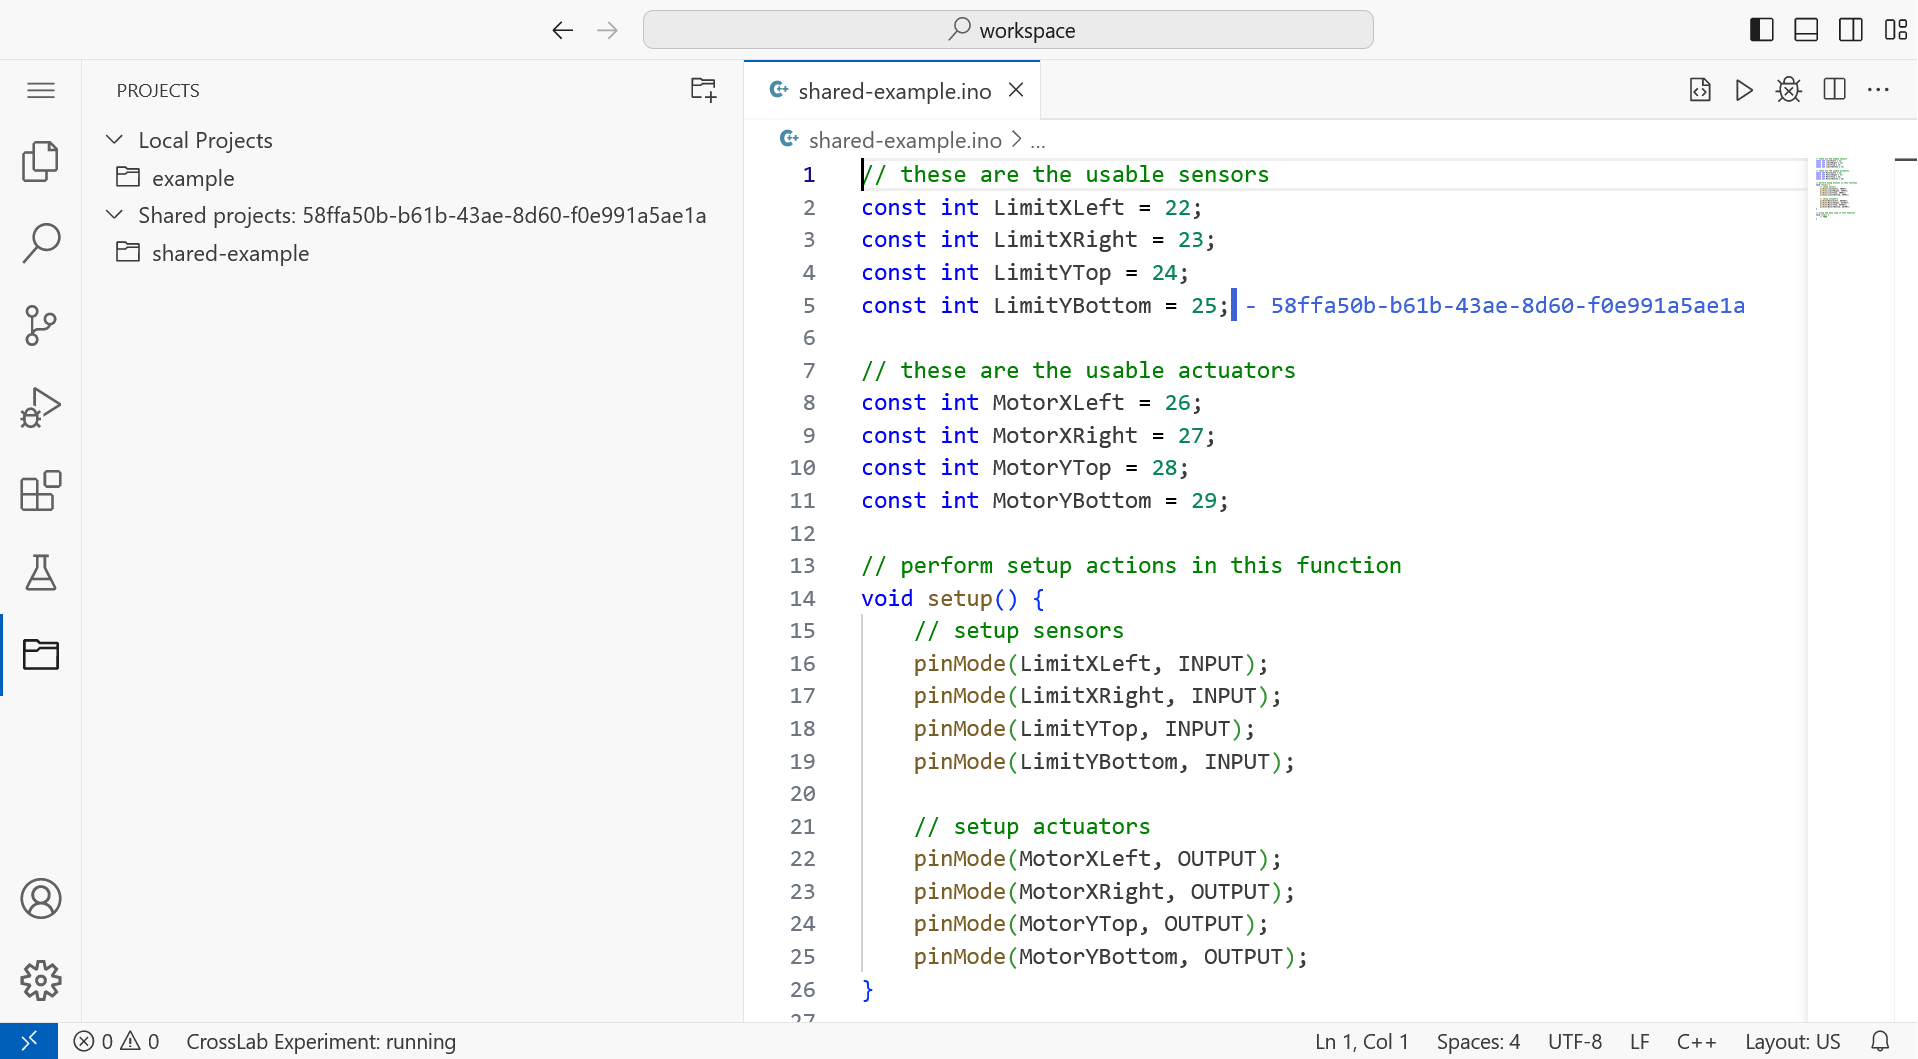
\includegraphics[trim={0 3px 0 0},clip,width=\textwidth]{images/projects-shared.png}
    \caption{Benutzerinterface der Projektverwaltung}
    \label{figure:benutzerinterface:dateisystem}
\end{figure}

Um die in \autoref{section:konzeption:dateisystem} beschriebenen Konzepte für die Bereitstellung und Nutzung von Dateisystemen umzusetzen, wurden der Filesystem Service sowie eine entsprechende Erweiterung für die IDE entwickelt. Diese Erweiterung wird im Folgenden als \textit{Filesystem Erweiterung} bezeichnet.

In \autoref{figure:klassendiagramm-dateisystem-service} ist ein Klassendiagramm für den Filesystem Service dargestellt. Der Filesystem Service Consumer besitzt die in \autoref{section:konzeption:dateisystem} genannten Funktionen zur Interaktion mit dem vom Filesystem Service Producer angebotenen Dateisystem. Der Filesystem Service Producer ermöglicht die Registrierung von Event-Handlern um auf die verschiedenen Anfragen reagieren zu können. Dadurch kann die Implementierung an das angebotene Dateisystem angepasst werden.

Die Filesystem Erweiterung ist für die Bereitstellung des integrierten Dateisystems und die Ermöglichung des kollaborativen Arbeitens an Programmen verwantwortlich. Für das integrierte Dateisystem wurde ein projektbasierter Ansatz gewählt. Dabei besitzen Nutzer mehrere verschiedene \textit{Projektordner}, deren direkte Unterordner als \textit{Projekte} bezeichnet werden. In der aktuellen Implementierung gibt es standardmäßig den Projektordner \texttt{/projects}. Die Projektordner sowie die enthaltenen Projekte werden dem Nutzer über ein entsprechendes Benutzerinterface angezeigt. Über dieses kann der Nutzer Projekte erstellen, öffnen, umbenennen und löschen. Für die Einbindung des Dateisystems wurde das Interface \texttt{FileSystemProvider} der VSCode Extension API implementiert. Für die Bereitstellung der Dateisystem-Funktionen können unterschiedliche \textit{Subprovider} verwendet werden. In der aktuellen Implementierung stehen dabei Subprovider für In-Memory, die Indexed Database API sowie den Filesystem Service zur Verfügung. Dabei werden standardmäßig der In-Memory Subprovider sowie der Indexed Database Subprovider für die persistente Speicherung der Projekte im Pfad \texttt{/projects} verwendet. Allerdings können der standardmäßig benutzte Subprovider sowie die Subprovider für bestimmte Pfade angepasst und neue Subprovider hinzugefügt werden. Weiterhin wurden auch die Schnittstellen \texttt{FileSearchProvider} und \texttt{TextSeachProvider} der VSCode Extension API implementiert, um es Nutzern zu ermöglichen, nach Dateien und Texten innerhalb des aktuellen Projekts zu suchen. Für das Benutzerinterface wurde eine \texttt{TreeView} verwendet, deren Daten über einen entsprechenden \texttt{TreeDataProvider} bereitgestellt werden. Das von der Filesystem Erweiterung bereitgestellte Benutzerinterface zur Verwaltung der Projekte ist in \autoref{figure:benutzerinterface:dateisystem} dargestellt. Dieses enthält auch bereits ein geteiltes Projekt, um die Darstellung unterschiedlicher Projektordner hervorzuheben.

Beim Öffnen eines neuen Ordners wird VSCode standardmäßig neugeladen. Dadurch werden auch alle Erweiterungen beendet und neugestartet, was dazu führt, dass das laufende Experiment beendet wird. Um dies zu vermeiden, muss der Wechsel von Projekten über einen anderen Mechanismus geschehen. Dazu wurde zunächst ein Pfad festgelegt, welcher standardmäßig von der IDE geöffnet wird. Im Falle der prototypischen Implementierung wurde der Pfad \texttt{/workspace} ausgewählt. Dieser Pfad nutzt standardmäßig einen In-Memory Subprovider. Sollte der Nutzer nun ein Projekt öffnen, wird von diesem Moment an der Pfad \texttt{/workspace} in allen URLs durch den Pfad des geöffneten Projektes ersetzt. Dadurch wird kein Neuladen der IDE ausgelöst und Nutzer können zwischen ihren Projekten wechseln. Das Umschreiben der Pfade führt allerdings zu Problemen beim Kopieren, Ausschneiden und Einfügen von Ordnern und Dateien. Daher müssen die entsprechenden Kommandos überschrieben werden, um die erwartete Funktionalität zu gewährleisten.

Um das Teilen von Projekten sowie das gleichzeitige Bearbeiten dieser zwischen Nutzern innerhalb eines Experiments zu ermöglichen, wurde eine entsprechende Komponente implementiert. Diese nutzt den \texttt{FileSystemProvider} sowie den von der Collaboration Erweiterung bereitgestellten Collaboration Service Prosumer. Über diesen wird ein enstsprechender Raum erstellt. Zu Beginn wird kein Projekt geteilt. Sobald ein Nutzer ein Projekt teilt, wird es zu dem geteilten Objekt des Raums hinzugefügt. Weiterhin werden auch Funktionen registriert, die auf Änderungen innerhalb des Projekts reagieren. Andere Nutzer die an der Kollaboration teilnehmen, können dann das geteilte Projekt über das bereitgestellte Benutzerinterface aufrufen. Alle Änderungen an Dateien und Ordnern werden zwischen den Nutzern synchronisiert. Weiterhin wird die aktuelle Position eines Nutzers innerhalb einer Datei über dessen Zustandsinformationen geteilt. Diese Position wird dann bei anderen Nutzern innerhalb derselben Datei markiert (siehe \autoref{figure:benutzerinterface:dateisystem}). Wenn der Besitzer des Projekts das Teilen beendet, wird das Projekt für alle anderen Nutzer geschlossen. Geteilte Projekte besitzen Pfade der Form \texttt{/shared/\{\{user\_id\}\}/\{\{project\_name\}\}}, wobei der Pfad \texttt{/shared} ein In-Memory Dateisystem verwendet. Die Projektordner \texttt{/shared/\{\{user\_id\}\}} werden automatisch erstellt, wenn ein Nutzer dem entsprechenden Raum beitritt.

Der betrachteten Experimentkonfiguration werden keine neuen Laborgeräte hinzugefügt. Die IDEs werden um einen Filesystem Service Consumer erweitert, der die Anbindung von weiteren Dateisystemen ermöglicht. Außerdem bieten die IDEs auch einen Filesystem Service Producer an, um die Nutzung des integrierten Dateisystems durch andere Laborgeräte zu ermöglichen (siehe \autoref{figure:experimentkonfiguration:dateisystem}). Zudem wird ein neuer Raum für die Verbindungen der Collaboration Service Prosumer hinzugefügt, um das Teilen von Projekten zu ermöglichen.